\documentclass[11pt]{article}

\usepackage[margin=1in]{geometry}
\usepackage[backend=biber,style=numeric,sorting=nyt]{biblatex}
\addbibresource{../references.bib}
\usepackage{amsmath,amssymb,amsfonts}
\usepackage{amsthm}
\usepackage{mathtools}
\usepackage{hyperref}
\usepackage{xr-hyper}
\usepackage{float}
% Pull labels from the technical companion (compile elements first).
% Minimal macros needed when importing external labels:
\newcommand{\Mcal}{\mathcal{M}}
\externaldocument[E-]{../elements/elements}
\providecommand{\Eref}[1]{\ref{E-#1}}
\providecommand{\Epageref}[1]{\pageref{E-#1}}
\usepackage{enumitem}
\usepackage{booktabs}
\usepackage{tikz}
\usetikzlibrary{arrows.meta,positioning,calc}

\newtheorem{definition}{Definition}

\newcommand{\R}{\mathcal{R}}

\title{Boundary--Interior Closure, Neutral Empiricism, and $\alpha$-Divergence Stances\\
\large A Programmatic Overview for Information Geometry \& Dynamical Systems}
\author{}
\date{}

\begin{document}
\maketitle

\begin{abstract}
We present a boundary-first empirical program for dynamical inference. The primitive data are
edge-level empirical objects (one-step marginals, and when available a multi-scale family across
time steps). Interior dynamical structure---Markov chains, Markov semigroups, infinitesimal generators,
and spectral elements---is treated as a \emph{completion} (a regularity closure) that is earned under

%==========================================================
\subsection{Worked example: local linear least squares with residual-derived noise}
\label{subsec:worked-example-lwls}

This example exhibits the program in its most concrete form: a
boundary-level empirical object (local stepwise conditionals), a
completion step (constructing a Markov kernel and testing closure), and
a continuous-time limit (a generator and its semigroup). The technical
counterpart is Example~\Eref{ex:lwls-residual-kernel} and
Lemma~\Eref{lem:scaling-regimes-generator} in the Elements document.

Given a time series $(x_k)_{k=0}^{N}\subset\R^d$ sampled at step
$\Delta t$, fix a query point $x$ and local weights $w_k(x)\ge 0$. Fit a
locally affine predictor by weighted least squares,
\[
  x_{k+1}\approx A(x)\,x_k + b(x),
\]
and define residuals $r_k=x_{k+1}-(A(x_k)x_k+b(x_k))$. A residual-derived
noise model (e.g.\ Gaussian) estimates a local covariance $\Sigma_{\Delta
t}(x)$ from the weighted residual second moment. This yields an explicit
data-driven Markov kernel
\[
  K_{\Delta t}(x,dy)=\mathcal N\!\bigl(y;\,\mu_{\Delta t}(x),\Sigma_{\Delta t}(x)\bigr)\,dy,
  \qquad \mu_{\Delta t}(x):=A(x)x+b(x),
\]
and hence a Markov operator $(T_{\Delta t}f)(x)=\int f(y)\,K_{\Delta t}(x,dy)$.

\paragraph{Completion as closure.}
Rather than assuming a Markov semigroup, we treat Markov structure as a
closure property to be \emph{tested}: does the family
$\{T_{\Delta t}\}$ approximately satisfy Chapman--Kolmogorov
composition at small steps, and does it possess a stable generator
limit as $\Delta t\to 0$? Divergences (including $\alpha$-divergences)
enter here as stance-dependent ways of measuring the deviation of
empirical multi-step conditionals from the composed kernel.

%----------------------------------------------------------
\subsection{Semigroup taxonomy from drift/noise scaling}
\label{subsec:semigroup-taxonomy}

In the LWLS construction the ``destination'' semigroup is determined by
the limiting generator, which is in turn controlled by the \emph{scaling
of drift and residual noise with $\Delta t$}. Different modeling choices
(and different empirical scaling regimes) therefore lead to different
familiar semigroup classes, summarized in
Table~\ref{tab:semigroup-taxonomy} (cf.\ Lemma~\Eref{lem:scaling-regimes-generator}).

\paragraph{Takeaway.}
The framework does not privilege a single interior dynamics class. It
explains which semigroup class is warranted by the \emph{boundary}
statistics (including scaling diagnostics), and it makes non-uniqueness
explicit when the boundary does not identify the interior uniquely.
explicit consistency and limiting conditions, rather than assumed a priori. This viewpoint offers a
systematic synthesis between reductionist and complexity approaches: reductionist structure is recovered
when completion succeeds; irreducible pluralism is acknowledged, but disciplined, when completion fails
or is non-unique. We also interpret Amari's $\alpha\in[-1,1]$ family of divergences as a parametric
family of \emph{empirical stances} governing which discrepancies are treated as epistemically costly,
and we propose practical diagnostics for selecting $\alpha$.
\end{abstract}

\section{The boundary--interior principle}
Many dynamical modeling pipelines implicitly begin with an \emph{interior} object---a latent state space,
equations of motion, or a Markov semigroup---and regard observations as a projection. In contrast, the
boundary-first program takes as primitive what is empirically stable and directly comparable across
representations: \emph{edge-level} statistical information.

\paragraph{Boundary data.}
Let $Y$ be an observation space and let $\Gamma_Y^{(\Delta t)} \in \mathcal P(Y\times Y)$ denote an
empirical stepwise marginal at scale $\Delta t$. When multiple scales are available we consider an
empirical family
\[
\{\Gamma_Y^{(\Delta t)}\}_{\Delta t\in(0,\Delta t_0]} \subset \mathcal P(Y\times Y),
\]
along with a reference/source law $\nu_Y\in\mathcal P(Y)$ and an information divergence $D_f$ (in
particular, Amari's $\alpha$-divergence family).

\paragraph{Interior structure as closure.}
An interior dynamical object (e.g.\ a continuous-time Markov semigroup) is not posited as ontology.
Instead, it is treated as a \emph{regularity closure problem}: when do the boundary data across scales
admit a coherent interior completion, and when do they not?

\paragraph{The ``necessary emptiness.''}
The gap between boundary data and an interior dynamics is not a deficiency of the framework; it is the
correct epistemic state in complex systems. Completion is possible only under additional, empirically
testable regularity. When completion fails or is non-unique, underdetermination is interpreted as an
empirically meaningful feature (not an error), and the framework seeks invariants and partial
comparability rather than forced uniqueness.

\section{Cathedral summary: one object, three layers}
The program is organized around a single core empirical object and three derived layers.

\subsection*{Core object (empirical, primitive)}
\begin{equation}
\Big(Y,\ \nu_Y,\ \{\Gamma_Y^{(\Delta t)}\}_{\Delta t\in(0,\Delta t_0]},\ D_f\Big).
\end{equation}

\subsection*{Layer A: neutral structure (always defined)}
From a fixed $\Gamma_Y^{(\Delta t)}$ one obtains canonical one-step structure (e.g.\ by disintegration)
and associated induced operators on a chosen space of observables. The \emph{neutral framework} then
organizes all realizations/factorizations compatible with the same boundary data into equivalence
classes (``leaves''), and identifies invariants that do not depend on a privileged latent ontology.

\subsection*{Layer B: completion (conditional, earned)}
\begin{itemize}[leftmargin=1.6em]
\item \textbf{Discrete-time:} A single $\Gamma_Y$ always yields a forward Markov extension (one-step kernel),
but a two-sided stationary completion requires an explicit balance/invariance condition on marginals.
\item \textbf{Continuous-time:} A Markov semigroup arises only as a limit completion of the family
$\{\Gamma_Y^{(\Delta t)}\}$ under semigroup-consistency and generator convergence conditions.
\end{itemize}

\subsection*{Layer C: spectral and geometric consequences (post-completion)}
Generator spectra, resolvents, eigen-elements, and long-time asymptotics are defined only after a
completion exists. Representation comparisons of spectral objects require (i) a neutral identification
mechanism and (ii) a shared completed dynamics.

\section{Edge germs, completions, and neutral invariants}
\label{sec:edge-germs}

The boundary data may be treated as a single mathematical object: a \emph{germ} of edge statistics at
small time scales. This packaging makes explicit (i) when an interior dynamics is determined,
(ii) when it is underdetermined, and (iii) which quantities remain meaningful in the absence of a
preferred completion.

\subsection{The edge germ}
Let $Y$ be a standard Borel space. Fix a reference/source law $\nu\in\mathcal P(Y)$ and a family of
edge marginals indexed by time scale,
\[
  \Gamma^{(\Delta t)} \in \mathcal P(Y\times Y), \qquad \Delta t\in(0,\Delta t_0],
\]
each with first marginal $\nu$. The associated \emph{edge germ} is
\begin{equation}
  \mathcal G_Y := \big(Y,\nu,\{\Gamma^{(\Delta t)}\}_{\Delta t\downarrow 0}\big).
  \label{eq:edge-germ}
\end{equation}
When only a single scale is available one may replace the germ by $(Y,\nu,\Gamma)$, but continuous-time
claims then require additional information.

\subsection{Completions as a (possibly empty) family}
An \emph{interior dynamics on $Y$} is a family of Markov kernels $\{P_t\}_{t\ge 0}$ with $P_0=\mathrm{Id}$
and $P_t\mathbf 1=\mathbf 1$ (and, when needed, strong continuity on a chosen observable space $X$).
Such an interior induces boundary edge marginals via
\begin{equation}
  \Gamma_{\{P_t\}}^{(\Delta t)}(dy,dy') := \nu(dy)\,P_{\Delta t}(y,dy').
  \label{eq:boundary-map}
\end{equation}
We write $\partial(\{P_t\}) := (Y,\nu,\{\Gamma_{\{P_t\}}^{(\Delta t)}\})$ for the induced edge germ.

\begin{definition}[Markov completion of an edge germ]
A \emph{(continuous-time) Markov completion} of $\mathcal G_Y$ is an interior dynamics $\{P_t\}_{t\ge 0}$
such that $\partial(\{P_t\})=\mathcal G_Y$, i.e.\ \eqref{eq:boundary-map} matches the empirical
$\Gamma^{(\Delta t)}$ for all $\Delta t$ in the germ. The set of completions is denoted
\[
  \mathrm{Comp}(\mathcal G_Y) := \big\{\{P_t\}_{t\ge 0} : \partial(\{P_t\})=\mathcal G_Y\big\}.
\]
\end{definition}

\paragraph{Necessary emptiness and underdetermination.}
In general $\mathrm{Comp}(\mathcal G_Y)$ may be empty or may contain multiple non-equivalent completions.
This expresses a precise form of ``necessary emptiness'': boundary data do not automatically determine a
unique interior dynamics. When a unique completion exists (up to standard equivalences), the framework
recovers a reductionist-style interior description; when it does not, the appropriate empirical output
is a structured description of the boundary object and its invariants.

\subsection{Neutral invariants and representation-independence}
Fix an information divergence $D_f$ (including Amari's $\alpha$-divergences). The divergence specifies a
geometry on spaces of boundary objects and thereby determines which distinctions are treated as
empirically meaningful. We write
\[
  \mathrm{Inv}_{D_f}(\mathcal G_Y)
\]
for the collection of quantities or structures computable from $\mathcal G_Y$ that are invariant under
admissible representation maps (e.g.\ coarse-grainings or sufficient statistics) that preserve the
relevant $D_f$-geometry. Conceptually, these are the stable empirical contents of the program even in
regimes where $\mathrm{Comp}(\mathcal G_Y)$ is empty or non-unique.

\subsection{Closure theorem schema (boundary \texorpdfstring{$\to$}{->} interior)}
The completion problem becomes well-posed once the germ carries sufficient multi-scale regularity. A
typical closure theorem has the following shape.

\begin{quote}
\textbf{Closure schema.} If the empirical family $\{\Gamma^{(\Delta t)}\}$ satisfies (i) an approximate
Chapman--Kolmogorov (semigroup-consistency) property as $\Delta t\downarrow 0$, (ii) a small-time
identity condition $\Gamma^{(\Delta t)}\Rightarrow \Delta_\#\nu$, and (iii) a generator-control
condition (expressed on a chosen observable space $X$) yielding a well-defined dissipative limit, then
$\mathrm{Comp}(\mathcal G_Y)\neq\varnothing$ and there exists a $C_0$ Markov semigroup
$\{P_t\}_{t\ge 0}$ whose skeleton matches the germ.
\end{quote}

Conversely, any $C_0$ Markov semigroup preserving $\nu$ induces an edge germ satisfying these boundary
regularity properties. In this sense, the existence of an interior semigroup is equivalent to boundary
regularity plus an explicit closure condition, once the functional setting is fixed.

\begin{table}[H]
\centering
\caption{How boundary-level drift/noise scaling selects the limiting Markov semigroup.}
\label{tab:semigroup-taxonomy}
\begin{tabular}{@{}p{0.27\linewidth}p{0.32\linewidth}p{0.33\linewidth}@{}}
\toprule
Boundary scaling signal & Limiting generator $L$ (informal) & Familiar semigroup / forward equation \\
\midrule
$\mathrm{Var}(\xi_{\Delta t}\mid x)=o(\Delta t)$ &
$Lf=a\cdot \nabla f$ &
Transport/Liouville semigroup; $\partial_t\rho + \nabla\!\cdot(a\rho)=0$ \\
\addlinespace
$\mathrm{Var}(\xi_{\Delta t}\mid x)=B(x)\Delta t+o(\Delta t)$ (Lindeberg) &
$Lf=a\cdot\nabla f + \tfrac12\mathrm{tr}(B\nabla^2 f)$ &
Diffusion / Fokker--Planck class; $\partial_t\rho = L^\ast\rho$
(heat, OU, Langevin as special cases) \\
\addlinespace
\textit{Heat:} $a=0$, $B=2\kappa I$ & $Lf=\kappa\,\Delta f$ & Heat semigroup; $\partial_t\rho=\kappa\,\Delta\rho$ \\
\textit{Ornstein--Uhlenbeck:} $a(x)=Ax$, $B$ const. & $Lf=(Ax)\cdot\nabla f + \tfrac12\mathrm{tr}(B\nabla^2 f)$ & OU semigroup; linear Fokker--Planck \\
\textit{Overdamped Langevin:} $a=-\nabla V$, $B=2\beta^{-1}I$ & $Lf=-\nabla V\cdot\nabla f + \beta^{-1}\Delta f$ & Langevin diffusion; Gibbs stationary density (when normalizable) \\
\addlinespace
Rare large increments; stable/jump scaling; L\'evy limit &
Integro-differential $L$ with L\'evy measure $\nu_x$ &
Jump/L\'evy semigroups; nonlocal forward equations
(e.g.\ fractional Laplacian when symmetric stable) \\
CK composition fails systematically at observed level &
No Markov closure on $x$ alone (needs latent state or enrichment) &
``No completion'' on this boundary; or a projected/approximate Markov model \\
\bottomrule
\end{tabular}
\end{table}


\paragraph{Recognition guide.}
In practice: (i) \emph{approximately linear} drift $a(x)\approx Ax$ with
\emph{nearly state-independent} covariance suggests an
Ornstein--Uhlenbeck (OU) limit; (ii) \emph{near-zero} drift with
\emph{isotropic} covariance suggests a heat (pure diffusion) limit; and
(iii) drift that is \emph{approximately a negative gradient}
$a(x)\approx -\nabla V(x)$ with $B\approx 2\beta^{-1}I$ suggests an
overdamped Langevin limit. Heavy-tailed/rare large increments indicate
jump (L\'evy) limits, while systematic Chapman--Kolmogorov failures
indicate that the observed variables do not close Markovianly (latent
state or enrichment required).

\section{What is resolved: a synthesis of reductionist and complexity approaches}
The boundary-first closure program offers a resolution/synthesis in the following sense:

\begin{enumerate}[leftmargin=1.8em]
\item \textbf{Reductionist structure is recovered when warranted.}
If the boundary family admits a stable completion (e.g.\ a $C_0$ Markov semigroup), one inherits the
full reductionist toolkit: generators, spectra, invariant measures, and mechanistic interpretation.

\item \textbf{Complexity pluralism is retained when necessary, but disciplined.}
When completion fails or is non-unique, the framework does not force a mechanism. Instead it supplies
structured comparability through neutral invariants, divergence geometry, and equivalence classes of
representations.

\item \textbf{Incommensurable model classes become comparable.}
Mechanistic, data-driven, and stochastic-closure models can be compared through a common currency:
their induced boundary objects $\Gamma_Y^{(\Delta t)}$ across scales and the divergence geometry on
the space of such objects.
\end{enumerate}

\section{Amari $\alpha$-divergences as empirical stances}
We adopt Amari's convention $\alpha\in[-1,1]$. Within this program, $\alpha$ is interpreted as a
\emph{stance parameter}: it encodes which direction of discrepancy is treated as epistemically costly,
and therefore what kind of closure is preferred in moving from boundary to interior.

\subsection{Three canonical stances}
\begin{itemize}[leftmargin=1.6em]
\item \textbf{$\alpha=0$ (structural realism / invariance-first).}
A neutral, self-dual stance emphasizing representation-stable structure. One privileges invariants
across admissible transformations and avoids directional bias between ``world-to-model'' and
``model-to-world'' mismatch.

\item \textbf{$\alpha\to +1$ (realist-leaning / coverage-first).}
A stance prioritizing coverage of observed transitions, including rare events. Epistemic cost is high
for models that under-assign probability to observed behavior. This tends to favor conservative
closures that do not rule out empirically observed edges.

\item \textbf{$\alpha\to -1$ (pragmatic / parsimony-first).}
A stance prioritizing sharpness, stability, and avoidance of unsupported transitions. Epistemic cost
is high for models that posit transitions not supported by boundary data. This often yields cleaner
coarse dynamics and more interpretable spectral structure, potentially at the cost of tail coverage.
\end{itemize}

\subsection{Empirical diagnostics for choosing $\alpha$}
The stance interpretation is not merely philosophical: it yields testable, data-driven criteria.
For a given $\alpha$, assess:
\begin{enumerate}[leftmargin=1.8em]
\item \textbf{Completion stability across scales:} does the family $\{\Gamma_Y^{(\Delta t)}\}$ satisfy
approximate semigroup consistency more strongly, and does a generator limit appear more stable?
\item \textbf{Spectral robustness:} are dominant spectral elements reproducible under resampling,
subsampling, or coarse-graining?
\item \textbf{Rare-event sensitivity:} does $\alpha$ materially change inferred tail transitions or
metastable structure? If so, is that variation stable and predictive, or noise-amplifying?
\item \textbf{Representation invariance:} are neutral equivalence classes (leaves) coherent and
stable under admissible maps, or brittle?
\end{enumerate}

\section{Figure: $\alpha$ as a stance parameter in boundary--interior closure}
Figure~\ref{fig:alpha-stances} summarizes the stance interpretation and its diagnostic consequences.

\begin{figure}[h]
\centering
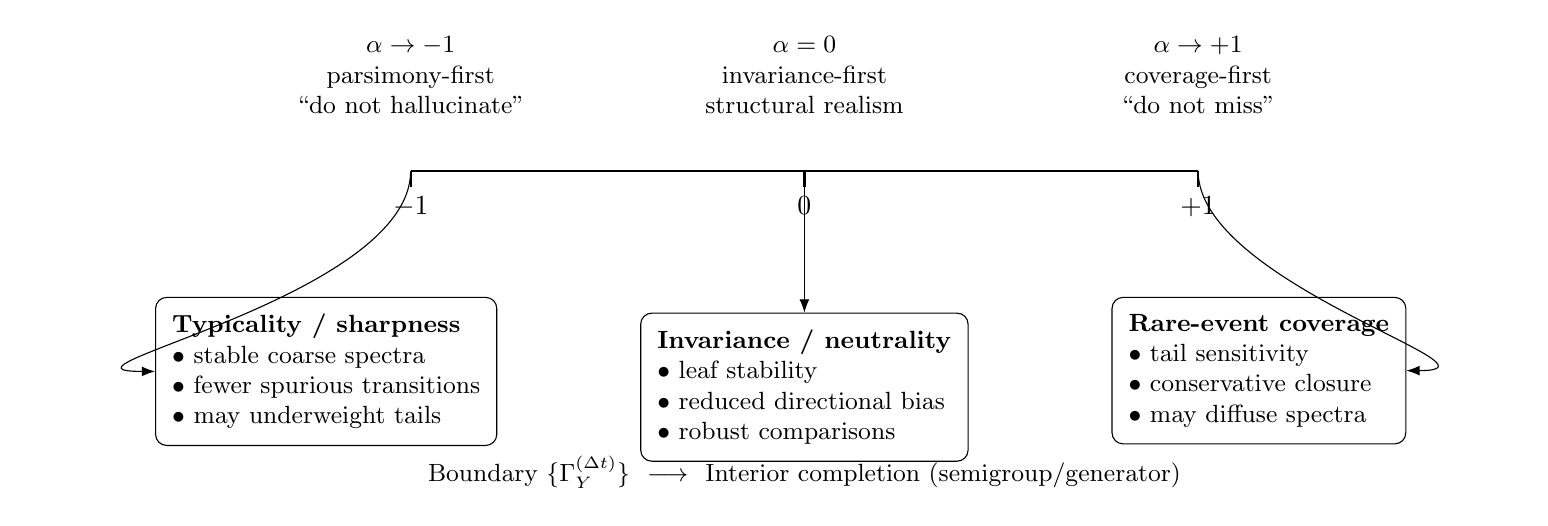
\begin{tikzpicture}[
  >=Latex,
  node distance=10mm,
  stance/.style={align=center, font=\small},
  box/.style={draw, rounded corners, inner sep=6pt, align=left, font=\small}
]
% Main alpha line
\draw[thick] (-5,0) -- (5,0);
\foreach \x/\lab in {-5/{$-1$}, 0/{$0$}, 5/{$+1$}}{
  \draw[thick] (\x,0) -- (\x,-0.2);
  \node[below] at (\x,-0.2) {\lab};
}

\node[stance, above=6mm] at (-5,0) {$\alpha\to -1$\\parsimony-first\\``do not hallucinate''};
\node[stance, above=6mm] at (0,0) {$\alpha=0$\\invariance-first\\structural realism};
\node[stance, above=6mm] at (5,0) {$\alpha\to +1$\\coverage-first\\``do not miss''};

% Arrows to diagnostic consequences
\node[box, below left=16mm and 2mm] (diagL) at (-3.7,0) {
\textbf{Typicality / sharpness}\\
$\bullet$ stable coarse spectra\\
$\bullet$ fewer spurious transitions\\
$\bullet$ may underweight tails
};
\node[box, below=16mm] (diagC) at (0,-0.2) {
\textbf{Invariance / neutrality}\\
$\bullet$ leaf stability\\
$\bullet$ reduced directional bias\\
$\bullet$ robust comparisons
};
\node[box, below right=16mm and 2mm] (diagR) at (3.7,0) {
\textbf{Rare-event coverage}\\
$\bullet$ tail sensitivity\\
$\bullet$ conservative closure\\
$\bullet$ may diffuse spectra
};

\draw[->] (-5,0) to[out=-90,in=180] (diagL.west);
\draw[->] (0,0) to[out=-90,in=90] (diagC.north);
\draw[->] (5,0) to[out=-90,in=0] (diagR.east);

% Boundary-interior label
\node[stance, below=35mm] at (0,0) {Boundary $\{\Gamma_Y^{(\Delta t)}\}$ \ $\longrightarrow$ \ Interior completion (semigroup/generator)};
\end{tikzpicture}
\caption{$\alpha$ as a stance parameter in the boundary--interior closure problem. Extremes
$\alpha\to\pm 1$ express directional risk preferences (parsimony vs coverage), while $\alpha=0$ emphasizes
representation-stable structure.}
\label{fig:alpha-stances}
\end{figure}

\section{Closing statement}
The boundary-first program reframes long-standing tensions between reductionist and complexity
approaches. Interior dynamics are not a precondition for inference, but a closure that may be earned
from multi-scale boundary data. Divergence choice---especially within Amari's $\alpha$-family---is
accordingly interpreted as an explicit empirical stance governing closure preferences, with empirical
diagnostics available to adjudicate these stances in practice.

\section*{Pointers to the technical companion}
This programmatic overview is intended to run in parallel with a technical ``elements'' document.
In particular, the neutral objects and completion-as-closure statements are made precise in
Definition~\Eref{def:neutral-operator} and the Markov completion sections
(see \S\Eref{subsec:markov-completion-discrete} and \S\Eref{subsec:markov-completion-continuous}),
with core invariance and embedding results collected in \S\Eref{sec:core-results}.

\vspace{1em}
\noindent\textbf{Acknowledgment of scope.} This document is intentionally programmatic: it sets the
architectural logic and interpretive stance. Technical statements (existence, uniqueness, stability of
completions; invariance theorems; spectral consequences) are to be supplied in the companion technical
manuscript once hypotheses and function-space choices are fixed.

\printbibliography

\end{document}